\documentclass{beamer}
\usepackage{amsmath,amsbsy,amsopn,amstext,amsfonts,amssymb}
\usepackage{isomath}
\usepackage{ulem}
%\linespread{1.6}  % double spaces lines
\usepackage{graphicx}
\usepackage{subfigure}
\usepackage{color}
\usepackage{optidef}  % define optimization problems
\usepackage{multicol}  % multiple columns
\usepackage{listings} % for python code
\usepackage{mathrsfs}

\usepackage{polynom}
\newcommand{\adj}{\mathrm{adj}}
\newcommand{\constrainedmin}[3]{
		\begin{mini*}|s|
		{#2}{#1}{}{}
		\addConstraint{#3}
		\end{mini*}
}

\newcommand{\rwbcomment}[1]{{\color{blue}RWB:#1}}
\newcommand{\defeq}{\stackrel{\triangle}{=}}
\newcommand{\abs}[1]{\left|#1\right|}
\newcommand{\norm}[1]{\left\|#1\right\|}
\newcommand{\iprod}[1]{\left<#1\right>}
\newcommand{\ellbf}{\boldsymbol{\ell}}
\newcommand{\nubf}{\boldsymbol{\nu}}
\newcommand{\mubf}{\boldsymbol{\mu}}
\newcommand{\abf}{\mathbf{a}}
\newcommand{\bbf}{\mathbf{b}}
\newcommand{\cbf}{\mathbf{c}}
\newcommand{\dbf}{\mathbf{d}}
\newcommand{\ebf}{\mathbf{e}}
\newcommand{\fbf}{\mathbf{f}}
\newcommand{\gbf}{\mathbf{g}}
\newcommand{\hbf}{\mathbf{h}}
\newcommand{\ibf}{\mathbf{i}}
\newcommand{\jbf}{\mathbf{j}}
\newcommand{\kbf}{\mathbf{k}}
\newcommand{\lbf}{\mathbf{l}}
\newcommand{\mbf}{\mathbf{m}}
\newcommand{\nbf}{\mathbf{n}}
\newcommand{\obf}{\mathbf{o}}
\newcommand{\pbf}{\mathbf{p}}
\newcommand{\qbf}{\mathbf{q}}
\newcommand{\rbf}{\mathbf{r}}
\newcommand{\sbf}{\mathbf{s}}
\newcommand{\tbf}{\mathbf{t}}
\newcommand{\ubf}{\mathbf{u}}
\newcommand{\vbf}{\mathbf{v}}
\newcommand{\wbf}{\mathbf{w}}
\newcommand{\xbf}{\mathbf{x}}
\newcommand{\ybf}{\mathbf{y}}
\newcommand{\zbf}{\mathbf{z}}
\newcommand{\Jbf}{\mathbf{J}}
\newcommand{\Acal}{\mathcal{A}}
\newcommand{\Bcal}{\mathcal{B}}
\newcommand{\Lcal}{\mathcal{L}}
\newcommand{\Ncal}{\mathcal{N}}
\newcommand{\Rcal}{\mathcal{R}}
\definecolor{darkolivegreen}{rgb}{0.33, 0.42, 0.18}

\makeatletter
\newenvironment<>{proofstart}[1][\proofname]{%
    \par
    \def\insertproofname{#1\@addpunct{.}}%
    \usebeamertemplate{proof begin}#2}
  {\usebeamertemplate{proof end}}
\newenvironment<>{proofcont}{%
  \setbeamertemplate{proof begin}{\begin{block}{}}
    \par
    \usebeamertemplate{proof begin}}
  {\usebeamertemplate{proof end}}
\newenvironment<>{proofend}{%
    \par
    \pushQED{\qed}
    \setbeamertemplate{proof begin}{\begin{block}{}}
    \usebeamertemplate{proof begin}}
  {\popQED\usebeamertemplate{proof end}}
\makeatother

\title{ECEn 671: Mathematics of Signals and Systems \\ 
Moon: Chapter 7.}
\author{Randal W. Beard}
\institute{Brigham Young University}
\date{\today}

\begin{document}

%-------------------------------
\begin{frame}
	\titlepage
\end{frame}

%-------------------------------
\begin{frame}[t]
\frametitle{Table of Contents}
\tableofcontents
\end{frame}

%%%%%%%%%%%%%%%%%%%%%%%%%%%%%%%%%%%%%%%%%%%%%%%%%%%%%%%%%%%%%%%%%
\section{Singular Value Decomposition}
\frame{\sectionpage}


%----------------------------------
\begin{frame}\frametitle{Singular Value Decomposition}
	\begin{theorem}[Moon Theorem 7.1]
		Every matrix $A \in \mathbb{C}^{m\times n}$ can be factored as $A = U\Sigma V^H$ where $U \in \mathbb{C}^{m\times m}$ and $V \in \mathbb{C}^{n\times n}$ are unitary and $\Sigma \in \mathbb{R}^{m\times n}$ is diagonal with diagonal elements $\sigma_1 \geq \sigma_2 \geq cdots \geq \sigma_p \geq 0$.
	\end{theorem}
	
	\vfill
		
	The diagonal elements are called the singular values of $A$.  If $A$ is real then $U$ and $V$ are real and orthogonal.
\end{frame}

%----------------------------------
\begin{frame}\frametitle{Singular Value Decomposition, Proof}
	Note that the $A^HA$ is Hermitian, and positive definite because $x^HA^HAx = \norm{Ax }^2 \geq 0 \qquad \forall x\in\mathbb{C}^n$.
	
	\vfill
	
	So, from Chapter 6 we know that the eigenvalues of $A^HA$ are real with $m_i = q_i$ for each $\lambda_i$.  
	
	\vfill
	
	Let $(\lambda_i,\vbf_i)$ be an eigenpairs of $A^HA$ then
	\[ 
		A^HAV = V\Lambda \qquad \qquad V \text{-unitary} 
	\]
	where 
	\[
		V = \begin{pmatrix}
	    		\vbf_1 & \cdots & \vbf_n
			\end{pmatrix}, 
		\qquad \qquad
		\Lambda = \begin{pmatrix}
	    			\lambda_1 & & 0\\
	   		 		& \ddots &\\
	    			0 & & \lambda_n
	  			  \end{pmatrix}, 
	  \]
	  with
	  \[
	  	\lambda_1 \geq \lambda_2 \geq \cdots \geq \lambda_n.
	  \]
	
\end{frame}

%----------------------------------
\begin{frame}\frametitle{Singular Value Decomposition, Proof}
	Since the $rank(A^HA) \leq \min(m,n) = p$, then number of non-zero eigenvalues is $r \leq p$.
	
	For $1 \leq i \leq r$ let $\ubf_i = \frac{A\vbf_i}{\sqrt{\lambda_i}}$.
	
	Then 
	\begin{align*}
		\iprod{\ubf_i,\ubf_j } &= \iprod{\frac{A\vbf_i}{\sqrt{\lambda_i}}, \frac{A\vbf_j}{\sqrt{\lambda_j}} }
		= \frac{1}{\sqrt{\lambda_i\lambda_j}}\vbf_i^HA^HA\vbf_j\\
		&= \frac{\lambda_j}{\sqrt{\lambda_i\lambda_j}}\vbf_i^H\vbf_j 
		=  \delta_{ij}
	\end{align*}
	Use Gram-Schmidt to extend $\ubf_1,\ldots,\ubf_r$ to $[\ubf_1,\ldots,\ubf_m]$ such that $U = [\ubf_1, \ldots \ubf_m]$ is unitary.

\end{frame}

%----------------------------------
\begin{frame}\frametitle{Singular Value Decomposition, Proof}
%	\begin{columns}
%		\begin{column}{0.5\linewidth}
		\begin{lemma}
			If $(\lambda_i, \vbf_i)$ is an eigenpair of $A^H A$, then 
			$\ubf_i=\frac{A\vbf_i}{\sqrt{\lambda_i}}$ are eigenvectors of  $AA^H$.
		\end{lemma}
		\begin{center}
			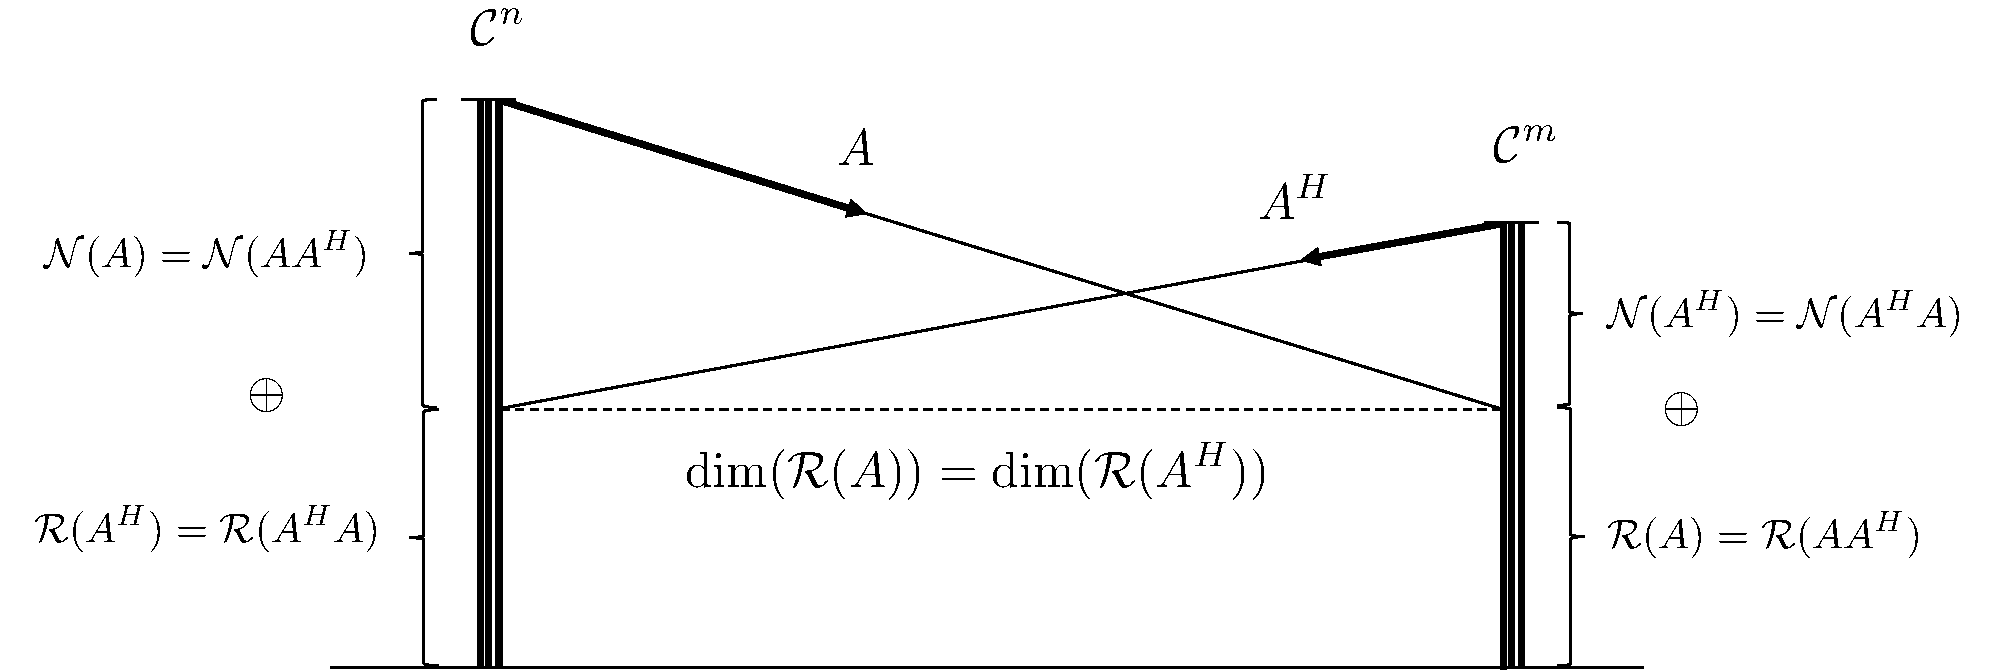
\includegraphics[width=0.5\textwidth]{figures/chap7_fundamental_subspace_1}
		\end{center}
%		\end{column}
%		\begin{column}{0.5\linewidth}
			\begin{proofstart}
				Note that since $\ubf_i = \frac{1}{\sqrt{\lambda_i}}A\vbf_i \qquad i = 1,\ldots,p$ then
				\begin{align*}
				& \ubf_i \in \mathcal{R}(A) \qquad i = 1, \ldots, p \\
				\implies & \ubf_i \in \mathcal{N}(A^H) \qquad i = p+1, \ldots, m \\
				\implies & \ubf_i \in \mathcal{N}(AA^H) \qquad i = p+1, \ldots, m \\
				\implies & AA^H\ubf_i = 0\cdot \ubf_i = 0 \\
				\implies & (0,\ubf_i) \text{~is an eigenpair of~} AA^H \qquad i = p+1,\ldots,m
				\end{align*}
			\end{proofstart}
%		\end{column}
%	\end{columns}
\end{frame}

%----------------------------------
\begin{frame}\frametitle{Singular Value Decomposition, Proof}
	Now lets look at
	\[ 
		U^HAV 
			= \begin{pmatrix}
	    		\ubf_1^H\\
	    		\vdots\\
	    		\ubf_m^H
	  		  \end{pmatrix}
	  		  A
	  		  \begin{pmatrix}
	    		\vbf_1 & \cdots & \vbf_n
	  		  \end{pmatrix} 
	  		= \begin{pmatrix}
	    		\ubf_1^HA\vbf_1 & \cdots & \ubf_1^HA\vbf_n\\
	    		\vdots & \ddots & \vdots\\
	    		\ubf_m^HA\vbf_1 & \cdots & \ubf_m^H\vbf_n
	  		  \end{pmatrix}.
	\]
	The $(i,j)^{th}$ element of $U^HAV$ is $\ubf_i^HA\vbf_j$.
	
	\vfill
	
	If $i \leq p$ then
	\begin{align*}
		\ubf_i^HA\vbf_j 
			&= \frac{1}{\sqrt{\lambda_i}}\vbf_i^HA^HA\vbf_j\\
			&= \frac{\lambda_j}{\sqrt{\lambda_i}}\vbf_i^H\vbf_j = \sqrt{\lambda_j}\delta_{ij}
	\end{align*}
\end{frame}

%----------------------------------
\begin{frame}\frametitle{Singular Value Decomposition, Proof}
	\begin{proofend}
		If $i > p$, then 
		\begin{align*}
			\ubf_i \in \mathcal{N}(A^H) &\Rightarrow A^H\ubf_i = 0 \\
			&\Rightarrow \ubf_i^HA = 0\\
			&\Rightarrow \ubf_i^H A \vbf_j = 0
		\end{align*}
		
		Therefore 
		\[
			U^HAV = \Sigma
		\]
		where $\Sigma = \text{diag}(\sigma_1, \ldots, \sigma_p)$ is real and diagonal, where $\sigma_j = 0$ when $j > p$.  Therefore
		\[
			A = U\Sigma V^H
		\] 
		as required.		
	\end{proofend}
\end{frame}

%----------------------------------
\begin{frame}\frametitle{Singular Value Decomposition}

	Note that the singular values of $A$ are the square root of the eigenvalues of $A^HA$ and $AA^H$.
	
	\vfill
	
	Also note that we can write 
	\[
	\Sigma 
		= \begin{pmatrix}
	    	\Sigma_1 & 0 \\
	    	0 & \Sigma_2
	  	  \end{pmatrix}
	  	= \begin{pmatrix}
 			\Sigma_1 & 0 \\
 			0 & 0	
 		  \end{pmatrix}
 	\]
	where
	\begin{align*}
		\Sigma_1 &= \underbrace{
						\text{diag}(\sigma_1, \dots, \sigma_p)
					}_{\mathbb{R}^{r\times r}} \\
		\Sigma_2 &= 0
	\end{align*}
\end{frame}

%----------------------------------
\begin{frame}\frametitle{Singular Value Decomposition}
	Then 
	\begin{align*}
	 A &= \begin{pmatrix}
	    	U_1 & U_2
	  	  \end{pmatrix}
	  	  \begin{pmatrix}
	    	\Sigma_1 & 0\\
	    	0 & 0
	      \end{pmatrix}
	      \begin{pmatrix}
	    	V_1^H\\
	    	V_2^H
	  	  \end{pmatrix}  \\
	&= \underbrace{U_1}_{m\times p}
	   \underbrace{\Sigma_1}_{p\times p}
	   \underbrace{V_1^H}_{n\times p} 
	   		\qquad \leftarrow\text{alternate form of SVD}\\
	&= \sum_{i=1}^p \sigma_i\ubf_i\vbf_i^H 
			\qquad \leftarrow\text{alternate form of SVD}
	\end{align*}	
	where $\ubf_i$'s are orthonormal and $\vbf_i$'s are orthonormal.
\end{frame}

%----------------------------------
\begin{frame}\frametitle{Singular Value Decomposition and Matrix Norm}
	Note that
	\begin{align*}
		\norm{A}_2 
			&= \sup_{\norm{x}_2=1}\norm{Ax}_2 
			= \sup_{\norm{x}_2=1}\sqrt{x^HA^HAx}\\
			&= \sup_{\norm{x}_2 = 1}\sqrt{x^HV_1\Sigma_1U_1^H U_1\Sigma_1V_1^Hx}\\
			&= \sup_{\norm{x}_2 = 1}\sqrt{x^HV_1\Sigma_1^2V_1^Hx}\\
			&= \sup_{\norm{x}_2 = 1}
				\sqrt{
					\begin{pmatrix}
		      			x^H\vbf_1 & \cdots & x^H\vbf_r
		    		\end{pmatrix}
		    		\begin{pmatrix}
		    			\sigma_1^2 & &\\
		    			& \ddots\\
		    			& & \sigma_p^2
		  			\end{pmatrix}
		  			\begin{pmatrix}
		    			\vbf_1^Hx\\
		    			\vdots\\
		    			\vbf_p^Hx
		  			\end{pmatrix}}  \\
		  	&= \sigma_1,
	\end{align*}	
	where the minimizer is $x = \vbf_1$.

\end{frame}

%----------------------------------
\begin{frame}\frametitle{Singular Value Decomposition and Rank}
	\begin{lemma}
		If $A \in \mathbb{C}^{m\times n}$, then 
		$\text{rank}(A) = p$ where $p$ is the number of non-zero singular values.
	\end{lemma}
	
	\begin{proof}
		\[ 
			\text{rank}(A) 
			= \text{rank}(U\Sigma V^H) 
			= \text{rank}(\Sigma) 
		\] 
		since $U$ and $V$ are both full rank.  
		Clearly $\text{rank}(\Sigma) = p$.
	\end{proof}
	
	
\end{frame}

%----------------------------------
\begin{frame}\frametitle{Singular Value Decomposition and Fundamental Subspaces}
	Fundamental subspace diagram:
	\begin{center}
		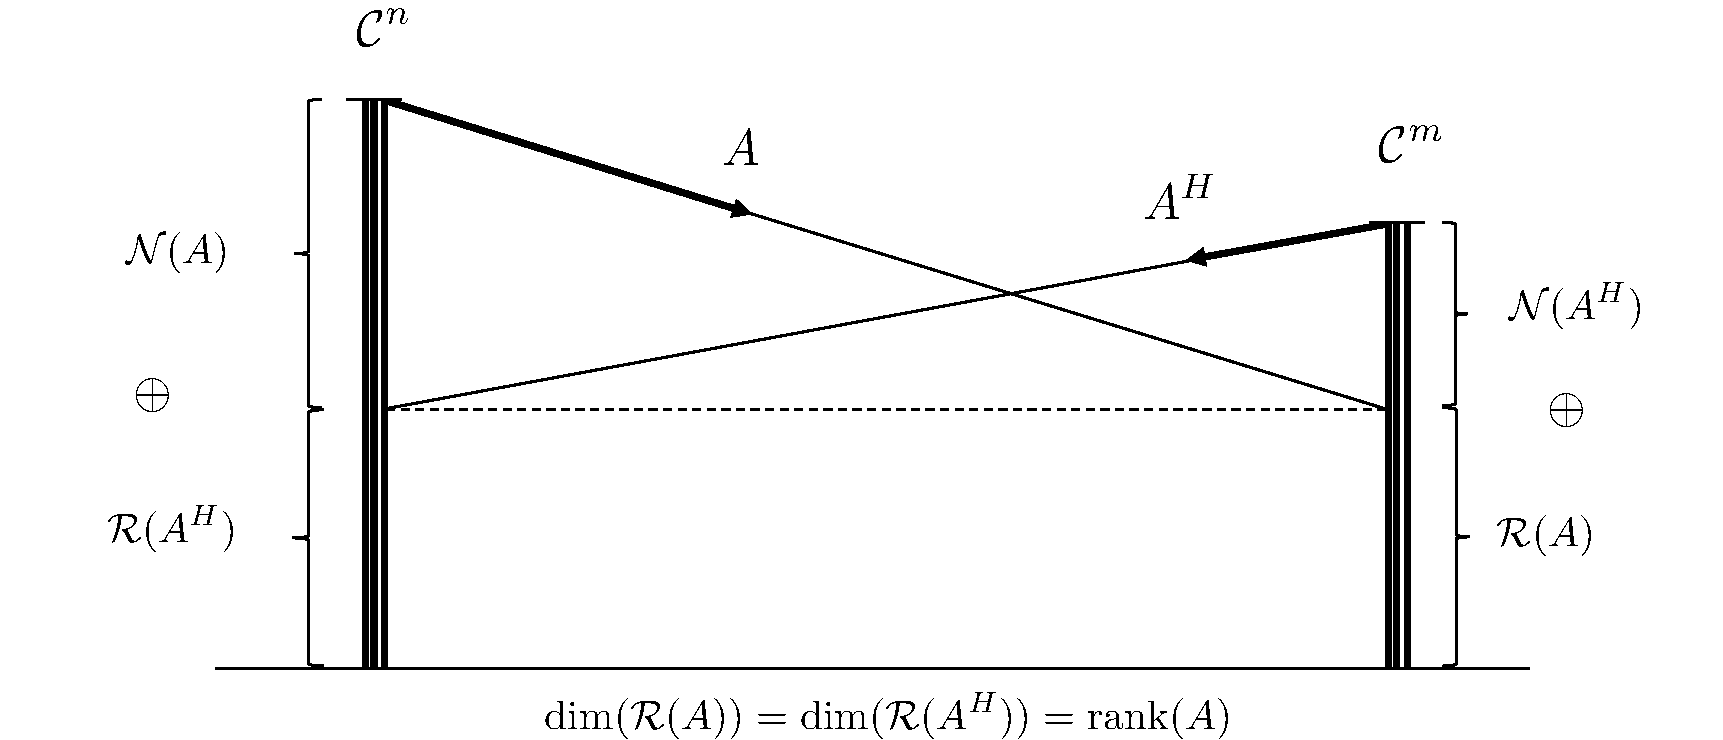
\includegraphics[width=0.9\textwidth]
			{figures/chap7_fundamental_subspace_2}
	\end{center}
	
	{\color{blue}Question:} 
		What information does the SVD provide?
		
	\vfill
	
	{\color{blue}Answer:} 
		The SVD completely characterizes all of the spaces.	
\end{frame}

%----------------------------------
\begin{frame}\frametitle{Singular Value Decomposition and Fundamental Subspaces}
	Given that 
	\[ 
		A = 
			\begin{pmatrix}
    			U_1 & U_2
  			\end{pmatrix}
  			\begin{pmatrix}
    			\Sigma_1 & 0\\
    			0 & 0
  			\end{pmatrix}
  			\begin{pmatrix}
    			V_1^H\\
    			V_2^H
  			\end{pmatrix}
  		= U_1\Sigma_1 V_1^H.
  	\]
	Let $y \in \mathcal{R}(A)$, then $\exists x \in \mathbb{C}^n$ such that $y = Ax$.  Which implies that 
	\begin{align*}
		y 
			&= U_1\Sigma_1V_1^Hx\\
			&= U_1z \text{ where } z = \Sigma_1V_1^Hx\\
			&= [\ubf_1 \cdots \ubf_p]
				\begin{pmatrix}
	    			z_1\\
	    			\vdots\\
	    			z_p
	  			\end{pmatrix} 
	  		= \ubf_1 z_1 + \cdots + \ubf_p z_p  \\
		\implies & y \in span\{\ubf_1, \cdots, \ubf_p\} \\
		\implies & \fbox{$\mathcal{R}(A) = span(U_1)$}
	\end{align*}
\end{frame}

%----------------------------------
\begin{frame}\frametitle{Singular Value Decomposition and Fundamental Subspaces}
	Since the columns of 
	$U_2$ 
	are orthonormal to 
	$U_1$ and 
	$\text{span}(U) = \mathbb{C}^m$ 
	and 
	$\mathcal{R}(A) \oplus \mathcal{N}(A^H) = \mathbb{C}^m$ 
	we must have that
	\[
		\fbox{$\mathcal{N}(A^H) = \text{span}(U_2)$}
	\]
	
	A similar argument shows that
	\[
		\fbox{$\mathcal{R}(A^H) = \text{span}(V_1)$}
	\]
	\[
		\fbox{$\mathcal{N}(A) = \text{span}(V_2)$}
	\]	
\end{frame}

%----------------------------------
\begin{frame}\frametitle{Singular Value Decomposition and Fundamental Subspaces}

	Therefore, the fundamental subspace diagram becomes
	\begin{center}
		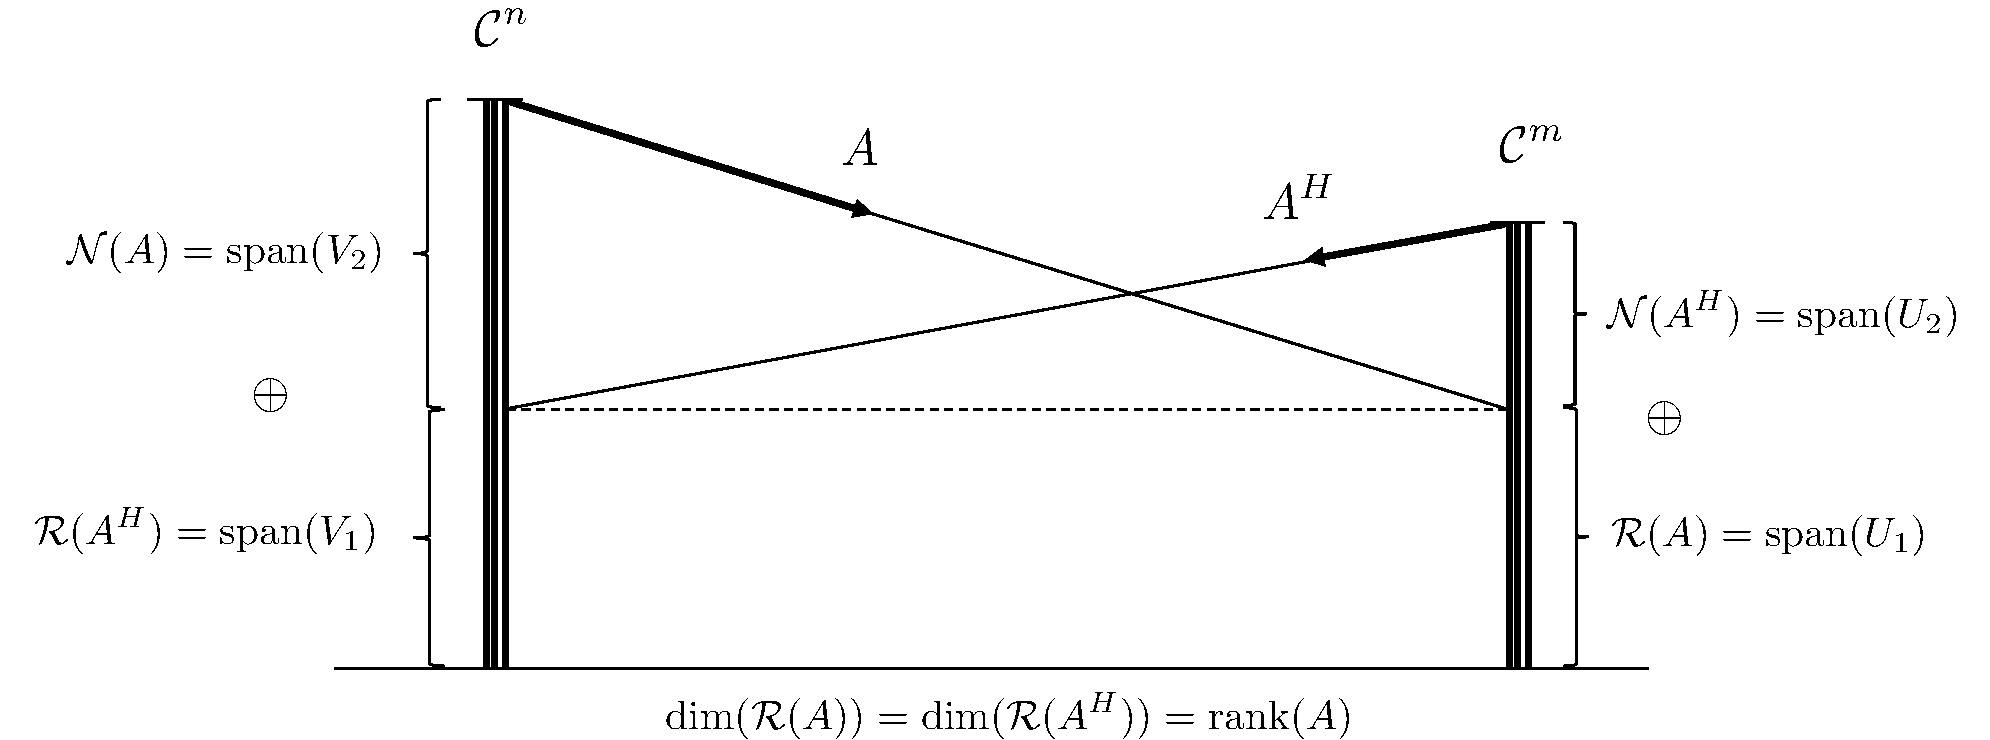
\includegraphics[width=0.99\textwidth]
			{figures/chap7_fundamental_subspace_3}	
	\end{center}
\end{frame}


%%%%%%%%%%%%%%%%%%%%%%%%%%%%%%%%%%%%%%%%%%%%%%%%%%%%%%%%%%%%%%%%%
\section{Pseudo Inverse and the SVD}
\frame{\sectionpage}

%----------------------------------
\begin{frame}\frametitle{Pseudo Inverses of $A$}
	Least squares solution to $Ax=b$ (i.e. $\min\norm{Ax-b}_2$) where $A$-tall is
	\[ 
		\hat{x} = (A^H A)^{-1} A^H b \defeq A^\dagger b.
	\]
	
	\vfill
	
	Minimum norm solution to $Ax = b$ (i.e. $\min\norm{x}$ for $Ax=b$) where $A$-fat is
	\[
		x = A^H (A A^H)^{-1} b \defeq A^\dagger b. 
	\]
	
	\vfill
	
	How does the SVD help compute the pseudo inverse.  We will consider both when $A$ is full rank, and when $A$ is not full rank.
\end{frame}

%----------------------------------
\begin{frame}\frametitle{SVD and Least Squared: Full Rank $A$}
	Assume $A\in\mathbb{C}^{m\times n}$ is tall, i.e.,  $m > n$, and that 
	$\text{rank}(A) = n$.  Then
	\[
		A = 
			\begin{pmatrix}
				U_1 & U_2	
			\end{pmatrix}
			\begin{pmatrix}
				\Sigma \\ 0	
			\end{pmatrix}
			V^H
		= U_1 \Sigma V^H
	\]
	where $U_1\in\mathbb{C}^{m\times n}$, $\Sigma \in \mathbb{R}^{n\times n}$, and $V\in\mathbb{C}^{n\times n}$.
	
	\vfill
	
	Then
	\begin{align*}
		(A^HA)^{-1}A^H 
			&= (V\Sigma U_1^HU_1\Sigma V^H)^{-1}V\Sigma U_1^H\\
			&= (V\Sigma^2V^H)^{-1}V\Sigma U_1^H\\
			&= V\Sigma^{-2}V^HV\Sigma U_1^H\\
			&= V\Sigma^{-1}U_1^H
	\end{align*}
	where $\Sigma^{-1} = \text{diag}(\frac{1}{\sigma_1}, \dots, \frac{1}{\sigma_n})$.	
\end{frame}

%----------------------------------
\begin{frame}\frametitle{SVD and min Norm: Full Rank $A$}
	Assume $A\in\mathbb{C}^{m\times n}$ is fat, i.e.,  $m < n$, and that $\text{rank}(A) = m$.  Then
	\begin{align*}
		A &= U \begin{pmatrix}
		      		\Sigma & 0
		    	\end{pmatrix}
		    	\begin{pmatrix}
		  			V_1^H\\
		  			V_2^H
				\end{pmatrix} \\ 
		&= U\Sigma V_1^H				
	\end{align*}
	where $U\in\mathbb{C}^{m\times m}$, 
	$\Sigma=\text{diag}(\sigma_1, \dots, \sigma_m)$, 
	$V_1 \in \mathbb{C}^{n\times m}$.
	
	\vfill
	
	Then 
	\begin{align*}
		A^H (A A^H)^{-1} 
			&= V_1 \Sigma U^H(U\Sigma V_1^HV_1\Sigma U^H)^{-1}\\
			&= V_1 \Sigma U^H(U\Sigma^2U^H)^{-1}\\
			&= V_1 \Sigma U^HU\Sigma^{-2}U^H\\
			&= V_1 \Sigma^{-1}U^H
	\end{align*}
	where $\Sigma^{-1} = \text{diag}(\frac{1}{\sigma_1}, \dots, \frac{1}{\sigma_m})$
\end{frame}

%----------------------------------
\begin{frame}\frametitle{SVD and Pseudo Inverse: Not Full Rank $A$}
	Assume $A\in\mathbb{C}^{m\times n}$ and that $\text{rank}(A) = p < \min(m,n)$.  Then
	\[ 
		A = 
			\begin{pmatrix} 
				U_1 & U_2	
			\end{pmatrix}
			\begin{pmatrix}
				\Sigma & 0 \\ 0 & 0	
			\end{pmatrix}
			\begin{pmatrix}
				V_1^H \\ V_2^H	
			\end{pmatrix}
		= U_1 \Sigma V_1^H
	\]
	where
	$U_1\in\mathbb{C}^{m\times p}$, 
	$\Sigma = \text{diag}(\sigma_1, \dots, \sigma_p) \in \mathbb{R}^{p\times p}$,
	$V_1 \in \mathbb{C}^{n \times p}$.

	Consider the least squares problem
	\begin{align*}
		\hat{x} &= (A^HA)^{-1}A^Hb\\
		&= (V_1\Sigma_1U_1^HU_1\Sigma_1V_1^H)^{-1}V_1\Sigma_1U_1^Hb\\
		&= (V_1\Sigma_1^2V_1^H)^{-1}V_1\Sigma_1U_1^Hb\\
		&= V_1\Sigma_1^{-2}V_1^HV_1\Sigma_1U_1^Hb\\
		&= V_1\Sigma_1^{-1}U_1^Hb
	\end{align*}
	where 
	$\Sigma_1 = \text{diag}(\frac{1}{\sigma_1}, \dots, \frac{1}{\sigma_p})$.
\end{frame}

%----------------------------------
\begin{frame}\frametitle{SVD and Pseudo Inverse: Not Full Rank $A$}
	So we can compute it, but what did we do?  How do we interpret the solution since the inverse of $A^HA$ does not exist?
	
	\begin{center}
		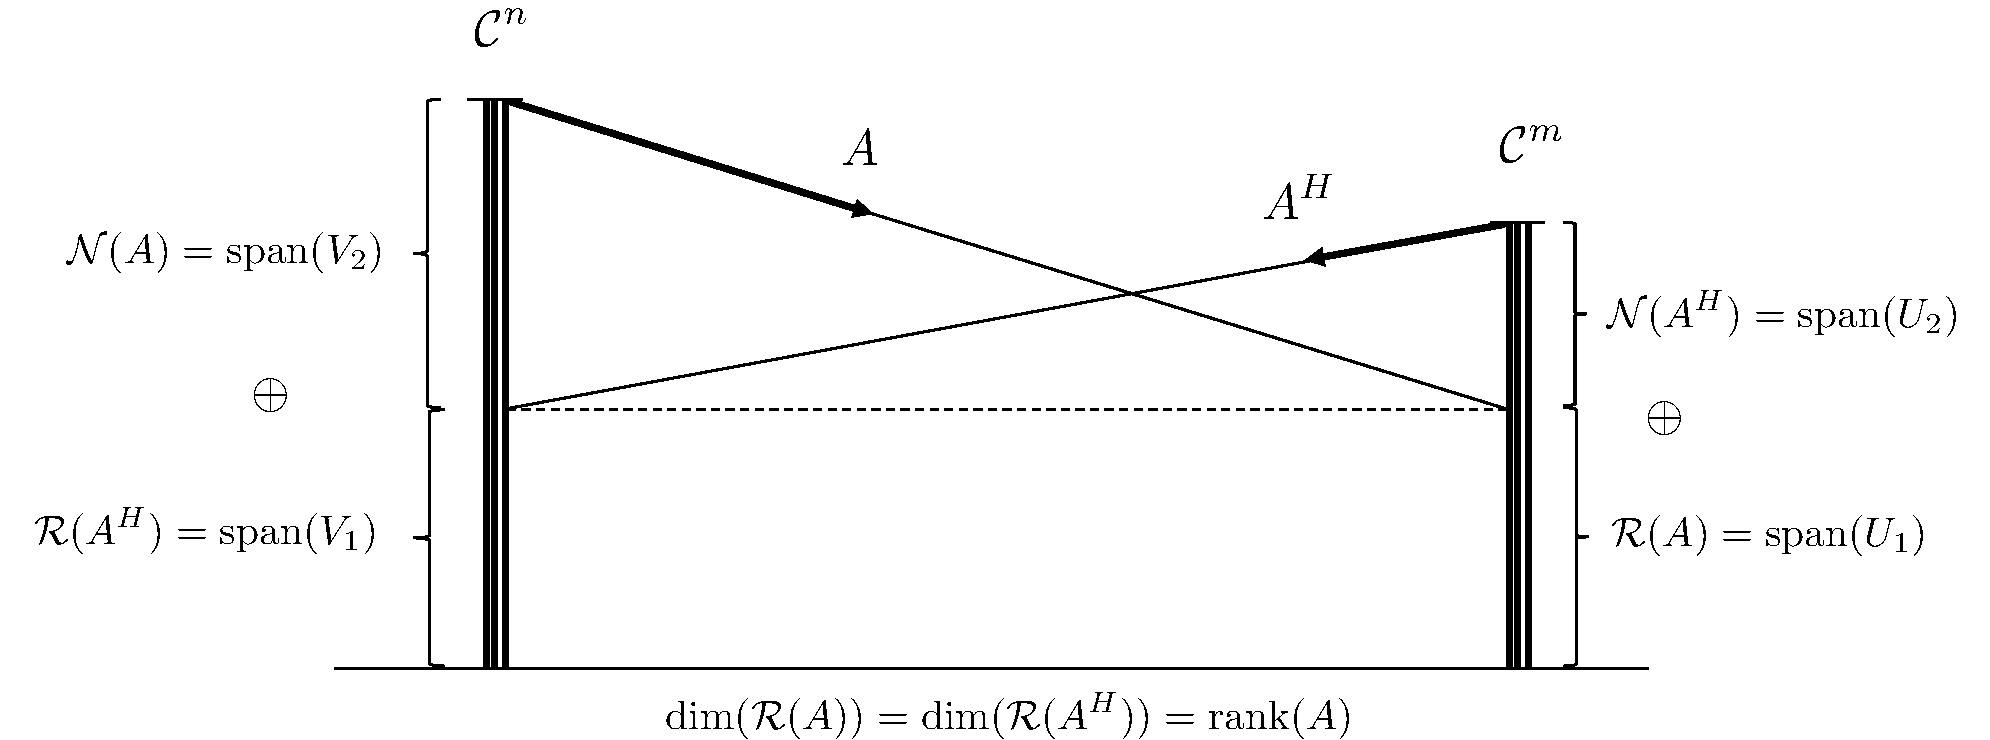
\includegraphics[width=0.9\textwidth]
			{figures/chap7_fundamental_subspace_3}
	\end{center}
	
	
	Find a solution to $Ax = b$ where $b \in \mathcal{R}(A)$.  But $\mathcal{N}(A)\neq \{0\}$ implies that there are more than one solution.
	
	\vfill
	
	Therefore, find the minimum norm $x$ that minimizes 
	$\norm{Ax - b}_2$.
\end{frame}

%----------------------------------
\begin{frame}\frametitle{SVD and Pseudo Inverse: Not Full Rank $A$}
	Note the following:
	\[ 
		\underbrace{U_1}_{m \times p}: \mathbb{C}^p \to \mathcal{R}(A) \subset \mathbb{C}^m
	\]
	so that
	\[ 
		U_1^\ast = U_1^H:\mathbb{C}^m\to\mathbb{C}^p.
	\]
	
	Also,
	\[ 
		\underbrace{V_1}_{n\times p}: \mathbb{C}^p \to 
			\mathcal{R}(A^H) \subset \mathbb{C}^n 
	\]
	so that
	\[ 
		V_1^H : \mathbb{C}^n \to \mathbb{C}^p.
	\]	
\end{frame}

%----------------------------------
\begin{frame}\frametitle{SVD and Pseudo Inverse: Not Full Rank $A$}
	So we have the following:
	\begin{center}
		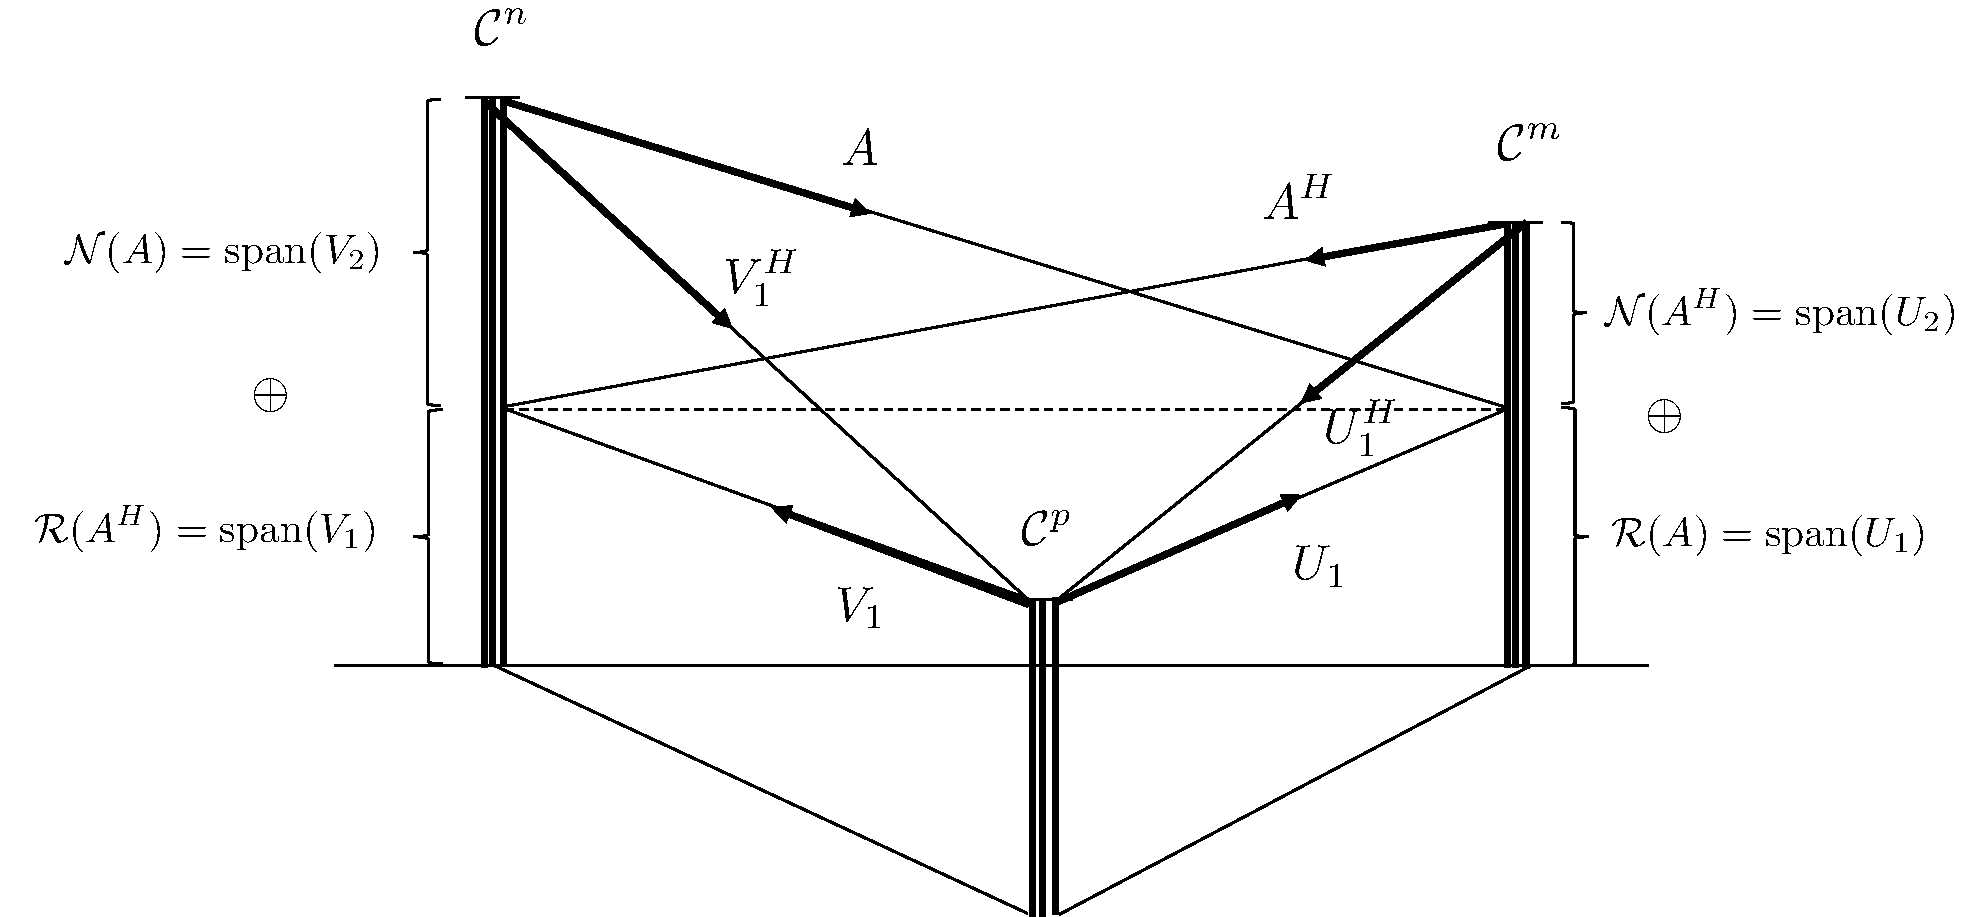
\includegraphics[width=0.9\textwidth]
			{figures/chap7_svd_1}
	\end{center}	
	Since $rank(A) = p$ we can only take inverses in 
	$\mathbb{C}^p$.  
	Therefore instead of solving $Ax=b$ directly in 
	$\mathbb{C}^n$ and 
	$\mathbb{C}^m$ we go indirectly through $\mathbb{C}^p$.
\end{frame}

%----------------------------------
\begin{frame}\frametitle{SVD and Pseudo Inverse: Not Full Rank $A$}
	\par\noindent{\color{blue}Step 1: Least Squares}
	
	Recall that to solve $\min\norm{Ax-b}_2$ when $A$ is full rank:
	\begin{center}
		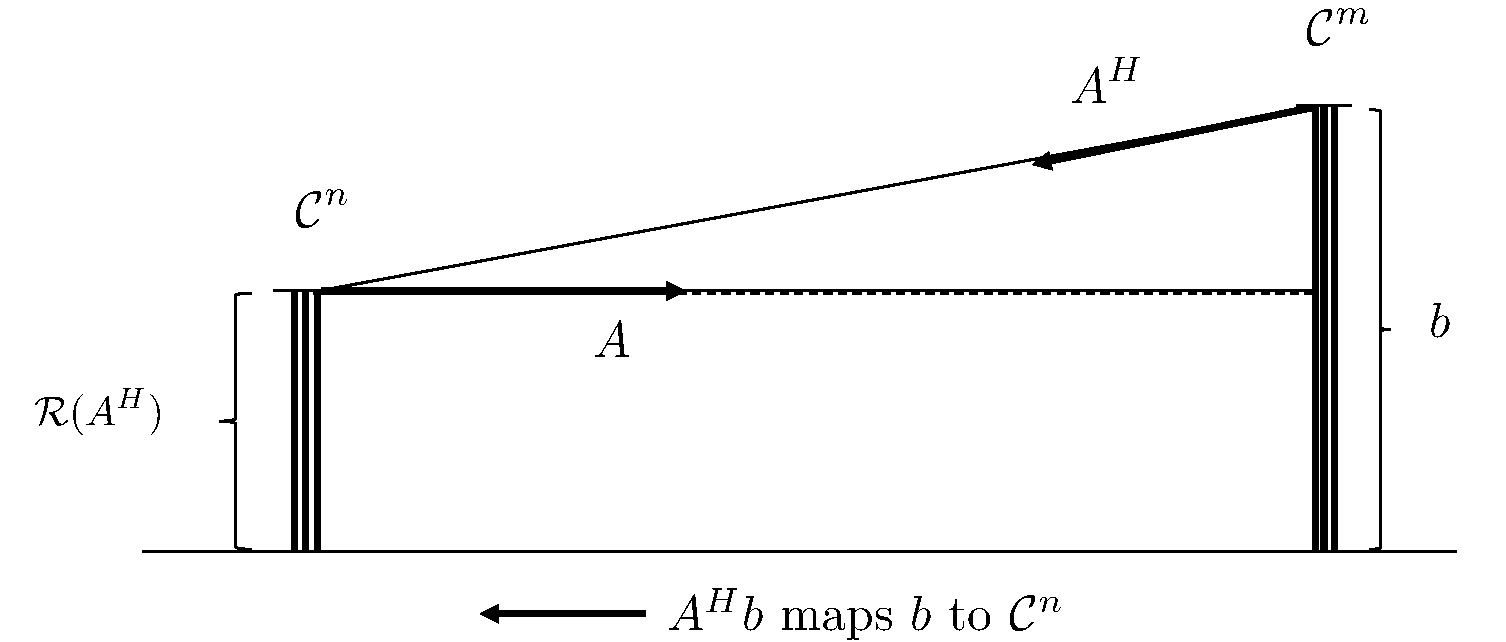
\includegraphics[width=0.9\textwidth]
			{figures/chap7_svd_2}
	\end{center}
	where we can invert things, i.e.
	\begin{align*}
		& A^HAx = A^Hb \\
		\implies & \hat{x} = (A^H A)^{-1} A^H b.
	\end{align*}
\end{frame}

%----------------------------------
\begin{frame}\frametitle{SVD and Pseudo Inverse: Not Full Rank $A$}
	So we have the following:
	\begin{center}
		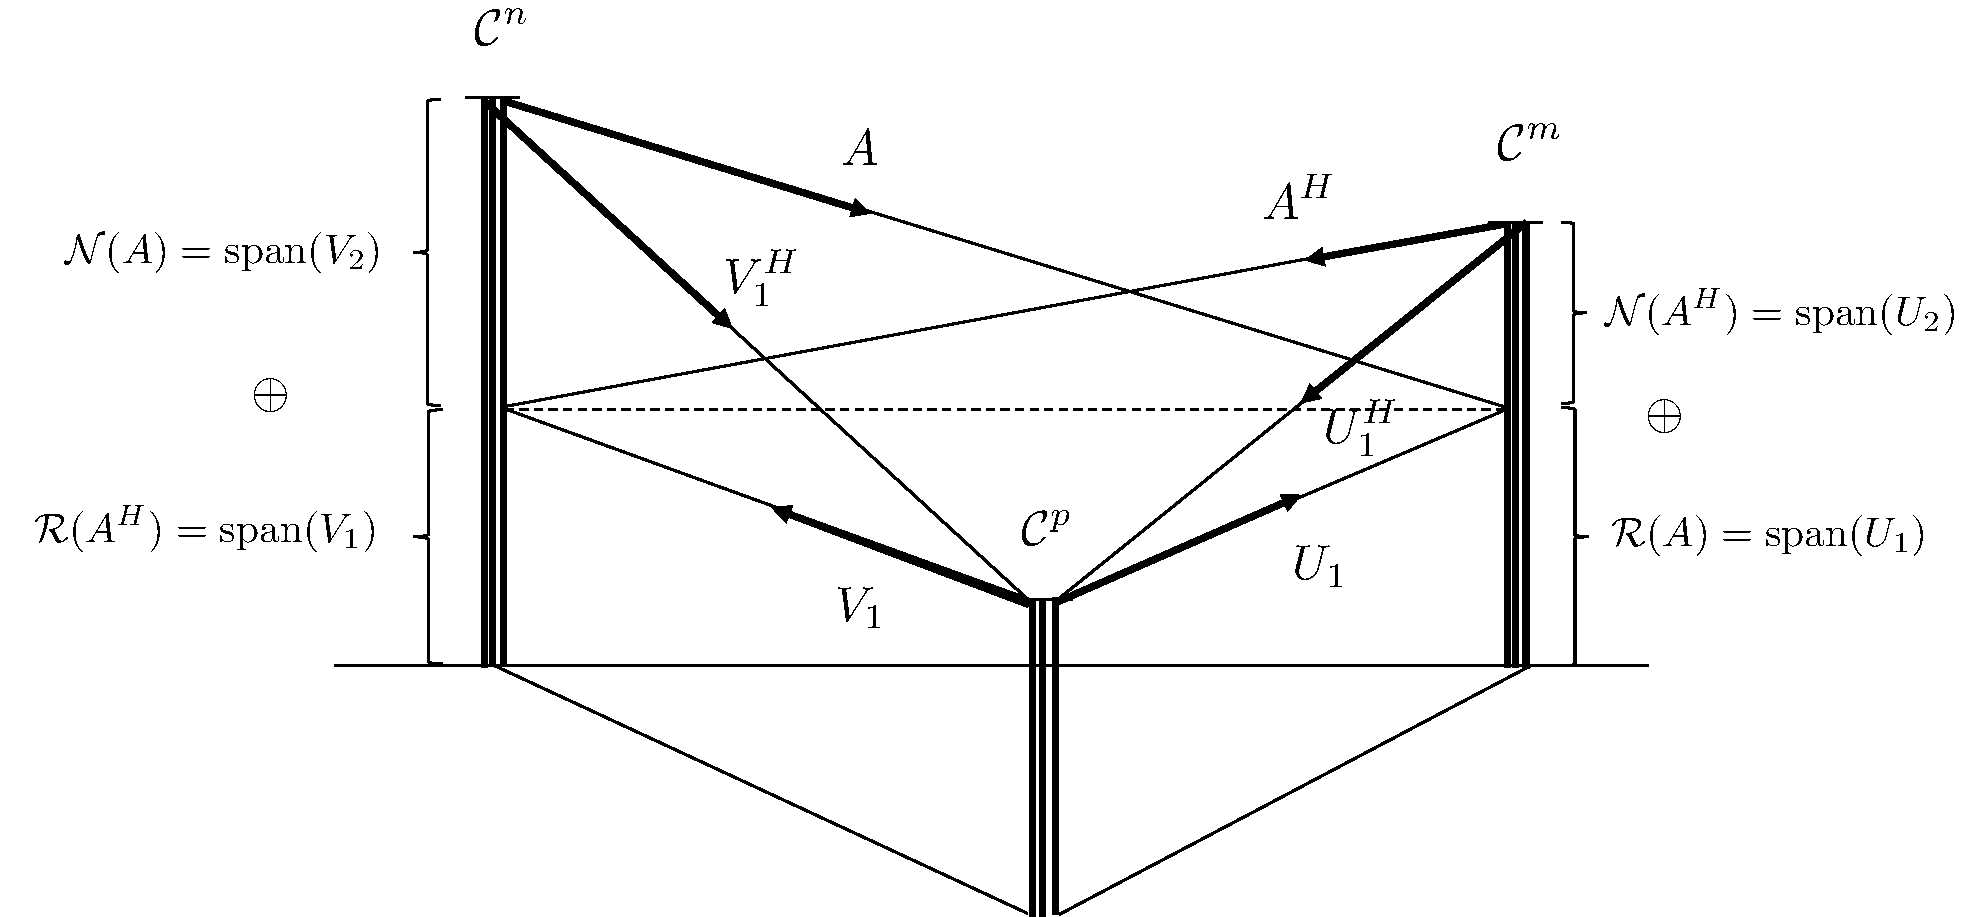
\includegraphics[width=0.9\textwidth]
			{figures/chap7_svd_1}
	\end{center}
	Now instead of $A^H$ we use $U_1^H$ to map to $\mathbb{C}^p$, i.e., given
	\[ 
		Ax = b
	\]
	map to $\mathbb{C}^p$ using $U_1^H$ to get:
	\[
		U_1^HAx = U_1^Hb \qquad \in\mathbb{C}^p.
	\]	
\end{frame}

%----------------------------------
\begin{frame}\frametitle{SVD and Pseudo Inverse: Not Full Rank $A$}
	\par\noindent{\color{blue}Step 2: Minimum Norm}
	
	Recall that to $\min\norm{x}$ such that $Ax = b$, $A$-full rank,
	\begin{center}
		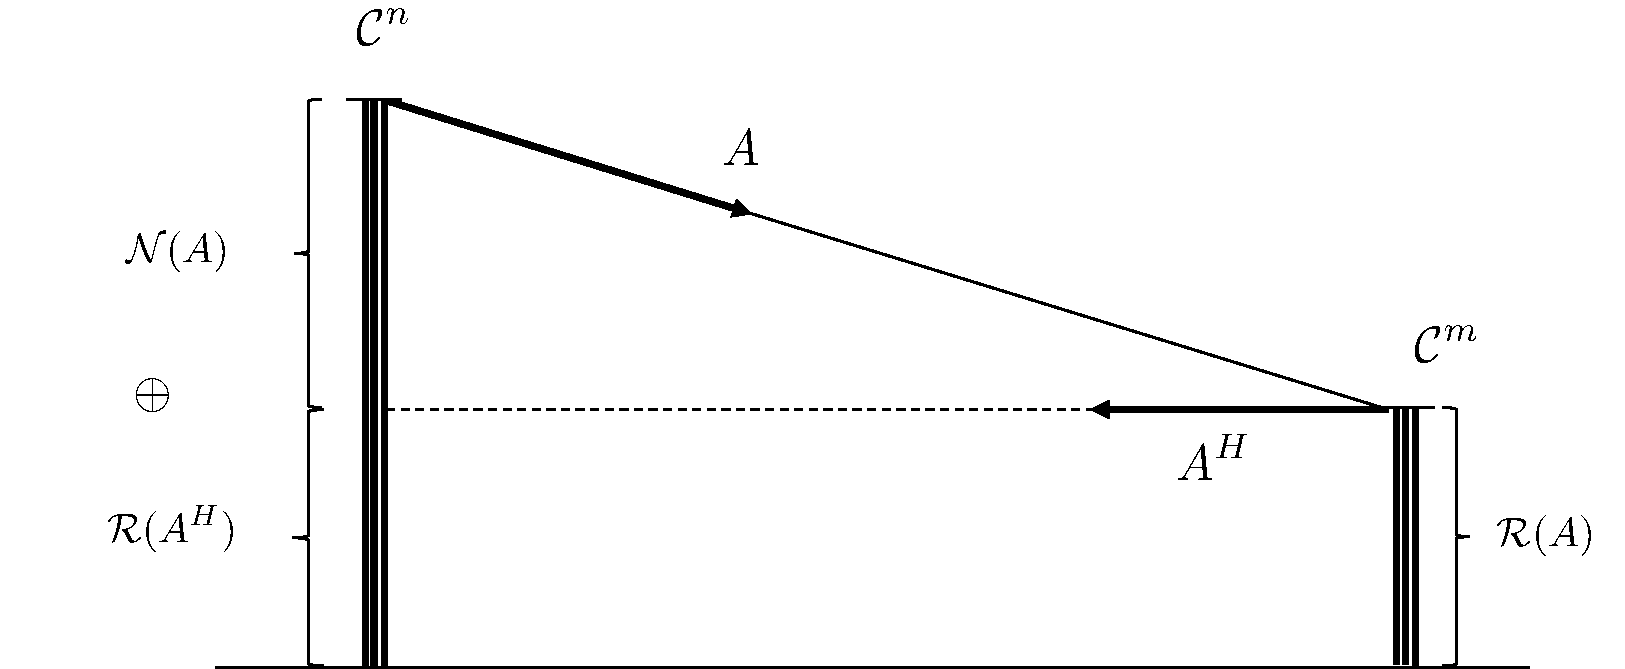
\includegraphics[width=0.7\textwidth]
			{figures/chap7_svd_3}
	\end{center}
	to minimize $\norm{x}$ we zero out the part that is in the null space of $A$, i.e. let
	\[ 
		x = A^Hz \text{ where } z \in \mathbb{C}^m 
	\]
	then
	\[ 
		AA^Hz = b 
		\qquad \Rightarrow \qquad 
		z = (AA^H)^{-1}b 
	\]
	so that
	\[ 
		\hat{x} = A^H(AA^H)^{-1}b.
	\]
\end{frame}

%----------------------------------
\begin{frame}\frametitle{SVD and Pseudo Inverse: Not Full Rank $A$}
	\begin{columns}
		\begin{column}{0.5\textwidth}
			In our case, again pick $x$ to zero the portion in the null space of $A$.  Let
			\[ 
				x = V_1z \quad \text{ where }  \quad z \in \mathbb{C}^p 
			\] 
			so that 
			\[ 
				U_1^HAx = \left(U_1AV_1\right) z = U_1^Hb. 
			\]	
			Note that 
			\[
				U_1AV_1: \mathbb{C}^p \to \mathbb{C}^p.
			\]
		\end{column}
		\begin{column}{0.5\textwidth}
			In fact,
			\[ 
				U_1^H A V_1 = U_1^H U_1 \Sigma_1 V_1^H V_1 = \Sigma_1.
			\]
			so we have
			\begin{align*}
				& \Sigma_1 z = U_1^Hb \\
				\implies & z = \Sigma_1^{-1}U_1^Hb \\
				\implies & \fbox{ $\hat{x} = V_1\Sigma_1^{-1}U_1^Hb$ }
			\end{align*}
			\begin{center}
				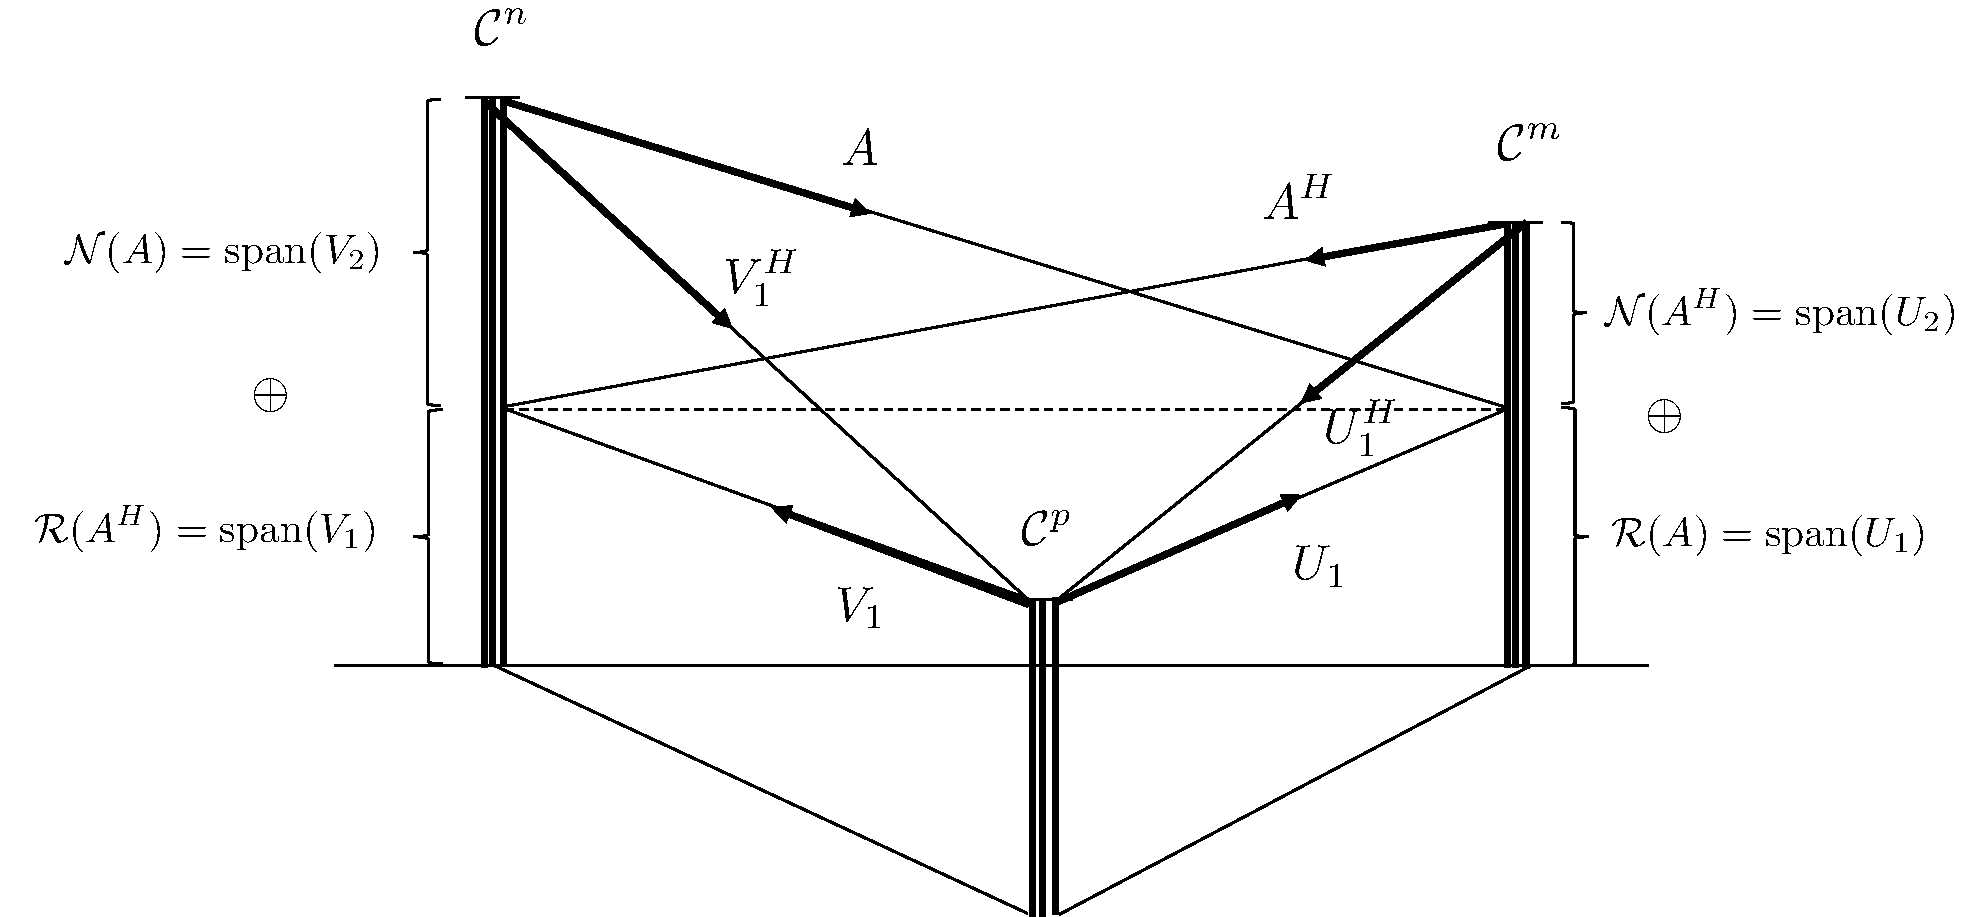
\includegraphics[width=0.9\textwidth]
					{figures/chap7_svd_1}
			\end{center}					
		\end{column}
	\end{columns}


	
\end{frame}

%%%%%%%%%%%%%%%%%%%%%%%%%%%%%%%%%%%%%%%%%%%%%%%%%%%%%%%%%%%%%%%%%
\section{SVD and Numerically Sensitive Problems}
\frame{\sectionpage}

%----------------------------------
\begin{frame}\frametitle{Numerically Sensitive Problems}
	Suppose that we would like to solve
	\[ 
		Ax = b  
	\]
	where $A \in \mathbb{R}^{n\times n}$ and $rank(A) = n$ but the condition number $\mathcal{K}(A)$ is large.  Let $A= U\Sigma V^H$, then 
	\begin{align*}
		 A^{-1} 
		 	&= V\Sigma^{-1} U^H\\
			&= \sum_{j=1}^{n}\frac{\vbf_j \ubf_j^H}{\sigma_j}
	\end{align*}
	
	so the solution to $Ax = b$ is
	\[ 
		x = A^{-1}b 
		  = \sum_{j=1}^{n}\frac{\vbf_j \ubf_j^H}{\sigma_j}.
	\]	
\end{frame}

%----------------------------------
\begin{frame}\frametitle{Numerically Sensitive Problems}
	Recall that 
	$\mathcal{K}(A) = \norm{A}\norm{A^{-1}}$ 
	where 
	$\norm{A} = \sigma_{\max}(A)$ 
	and 
	$\norm{A^{-1} } = \displaystyle\frac{1}{\min_{\norm{x}}\norm{A}} = \frac{1}{\sigma_{\min}(A)}$. 
		Therefore
	\[
		\mathcal{K}(A) = \frac{\sigma_{\max}(A)}{\sigma_{\min}(A)}
	\]
	
	\vfill
	
	Therefore a large $\mathcal{K}(A)$ implies there is significant difference between the largest and smallest singular values.	
\end{frame}

%----------------------------------
\begin{frame}\frametitle{Numerically Sensitive Problems}
	For example $\sigma_{\min}(A)$ may be very small, therefore given 
	\[ 
		x = \sum_{j=1}^n \frac{\vbf_j\ubf_j^H}{\sigma_j}b 
	\]
	x is very sensitive to small change in $b$ due to the terms in the sum that have very small singular values.	
	
	\vfill
	
	{\color{blue}Solution:}  
	Zero out small singular values to get the approximate solution
	\[ 
		Ax = \begin{pmatrix}
	  			U_1 & U_2  
			 \end{pmatrix}
			 \begin{pmatrix}
	    		\Sigma_1 & 0\\
	    		0 & \Sigma_2
	  		 \end{pmatrix}
	  		 \begin{pmatrix}
	    		V_1^H\\
	    		V_2^H
	  		 \end{pmatrix} x 
	  	\approx \begin{pmatrix}
	    			U_1 & U_2
	  			\end{pmatrix}
	  			\begin{pmatrix}
	    			\Sigma_1 & 0\\
	    			0 & 0
	  			\end{pmatrix}
	  			\begin{pmatrix}
	    			V_1^H\\
	    			V_2^H
	  			\end{pmatrix} x
	\]
	so
	\[ 
		x = V_1\Sigma_1^{-1}U_1^Hb 
	\]
	is an approximate solution that is numerically stable.
\end{frame}

%----------------------------------
\begin{frame}\frametitle{Numerically Sensitive Problems}
	\begin{itemize}
		\item Moon Example 7.4.1 shows that if $\sigma_j$-small then the vector $\ubf_j \in \mathbb{R}^m$ defines a sensitive direction for $b$.  i.e. if $b$ is almost parallel with $\ubf_j$ then $x = \frac{\vbf_j\ubf_j^H}{\sigma_j}b$ is clearly sensitive to small changes in $b$.  If $b$ is perpendicular to $\ubf_j$ then $\ubf_j^Hb=0$ and we are ok.
		\item If $A$ comes from noisy data (almost always) then $A$ will usually be full rank, even if the original data that produced $A$ would have resulted in a lower rank $A$ if it wasn't corrupted by noise.
		\item But the nonzero singular values added by noise will usually be small.
		\item Therefore, an effective way to reduce the rank of $A$ to get rid of the effect of noise is to zero the ``small'' singular values.
	\end{itemize}
\end{frame}


%%%%%%%%%%%%%%%%%%%%%%%%%%%%%%%%%%%%%%%%%%%%%%%%%%%%%%%%%%%%%%%%%
\section{Rank Reducing Approximations}
\frame{\sectionpage}

%----------------------------------
\begin{frame}\frametitle{Rank Reducing Approximations}
	{\color{blue}Problem:}  Given $A$ with $rank(A) = r$, find a matrix $B$ that is ``close'' to $A$ in some sense, but with lower rank.	
	
	\begin{theorem}[Moon Theorem 7.2]	
		Given $A \in \mathbb{C}^{m\times n}$ with $rank(A)=r$, then
		\[
			A = U_1\Sigma_1V_1^H = \sum_{j=1}^r \sigma_j\ubf_j\vbf_j^H
		\]
		
		Let $k < r$ and let 
		\[ 
			A_k \defeq \sum_{j=1}^k\sigma_j\ubf_j\vbf_j^H \qquad (rank(A_k) = k) 
		\]
		
		Then $\norm{A-A_k}_2 = \sigma_{k+1}$ and $A_k$ is the nearest rank $k$ matrix to $A$, in the matrix 2-norm, i.e.
		\[ 
			A_k = \arg\min_{rank(B)=k} \norm{A-B }_2.
		\]
	\end{theorem}
\end{frame}

%----------------------------------
\begin{frame}\frametitle{Rank Reducing Approximations, Proof}
	{\color{blue}Remark:} In the previous section, we saw that we could reduce the rank by zeroing small singular values.  This theorem shows that this is the best way to reduce the rank in the matrix 2-norm sense.	

	\begin{proofstart}
		\begin{align*}
			\norm{A-A_k }_2 
				&= \norm{\sum_{j=k+1}^r\sigma_j\ubf_j\vbf_j^H }_2 \\
				&= \max_{\norm{x }=1}\norm{\sum_{j=k+1}^r\sigma_j\ubf_j\vbf_j^Hx }_2
		\end{align*}
		Note that we maximize by letting $x^\ast = \vbf_{k+1}$ since any other $x$ will be a linear combination of smaller singular values.	
	\end{proofstart}
\end{frame}

%----------------------------------
\begin{frame}\frametitle{Rank Reducing Approximations, Proof}
	Therefore
	\[ 
		\norm{A-A_k} = \norm{\sigma_{k+1 }\ubf_{k+1}} = \sigma_{k+1} 
	\]
	since $\norm{\ubf_{k+1}} = 1$.
	
	\vfill
	
	Because $\norm{A-A_k }_2 = \sigma_{k+1}$ we know that
	\[ 
		\min_{rank(B)=k}\norm{A-B } \leq \sigma_{k+1}.
	\]
	To complete the proof we need to show that
	\[ 
		\sigma_{k+1} \leq \min_{rank(B)=k}\norm{A-B }.
	\]	
\end{frame}

%----------------------------------
\begin{frame}\frametitle{Rank Reducing Approximations, Proof}
	Let $B$ be any rank-$k$ matrix.  Then 
	\[
		rank(B)=k \quad \implies \quad dim(\mathcal{N}(B))=n-k.
	\]
	Therefore, there exists $ \{x_{k+1},\ldots,x_n\} $ such that
	\[ 
		\mathcal{N}(B) = span\{x_{k+1}, \ldots, x_n \}
	\]
	The columns of $V_1$ are $\{\vbf_1\ldots \vbf_k,\vbf_{k+1}\ldots \vbf_r\}$ where $\vbf_i \in \mathbb{C}^n$.
	Let 
	\[
		z \in 
			\underbrace{
				span\underbrace{
						\{x_{k+1},\ldots,x_n\}
					}_{dim=n-k} 
					~~\cap~~ 
				span\underbrace{
						\{\vbf_1,\ldots,\vbf_{k+1}\}
					}_{dim=k+1}
			}_{\text{dimension at least one since there are $n+1$ vectors}
			} 
	\]
	Therefore $z \neq 0$.
\end{frame}

%----------------------------------
\begin{frame}\frametitle{Rank Reducing Approximations, Proof}
	Let 
	\begin{align*}
		\norm{A-B }_2 
			&= \max_{\norm{x }\neq 0}\frac{\norm{(A-B)x }}{\norm{x }} \leq \frac{\norm{(A-B)z }}{\norm{z }} \\
			&= \frac{\norm{Ax }}{\norm{z }} \text{ since } z \in \mathcal{N}(B) \\
			&= \frac{\norm{\sum_{j=1}^r\sigma_j\ubf_j\vbf_j^Hz }}{\norm{z }} = \frac{\norm{\sum_{j=1}^{k+1}\sigma_j\ubf_j\vbf_j^Hz }}{\norm{z }}
	\end{align*}	
	Since $z \perp span\{\vbf_{k+2},\ldots,\vbf_r\}$ the smallest we can make the numerator is $\sigma_{k+1}$ by a choice of $z = \vbf_{k+1}$.  So
	\[ 
		\norm{A-B }_2 
			\geq \frac{\norm{\sigma_{k+1 }\vbf_{k+1}}}{\norm{\vbf_{k+1} }} 
			= \sigma_{k+1} 
	\]
	for any $B$ such that $rank(B) = k$ so that
	\[ 
		\min_{rank(B) = k}\norm{A-B }_2 \geq \sigma_{k+1}.
	\]
\end{frame}

%%%%%%%%%%%%%%%%%%%%%%%%%%%%%%%%%%%%%%%%%%%%%%%%%%%%%%%%%%%%%%%%%
\section{Applications}
\frame{\sectionpage}

%----------------------------------
\begin{frame}\frametitle{Application:  Total least squares}
	If we are trying to fit a line to
	\[ 
		y_i = ax_i
	\]
	where $(y_i,x_i)$ are measured.  The least squares solution minimizes $e_i = y_i-ax_i$.
	Therefore $y_i - e_i = ax_i$.
	\begin{center}
		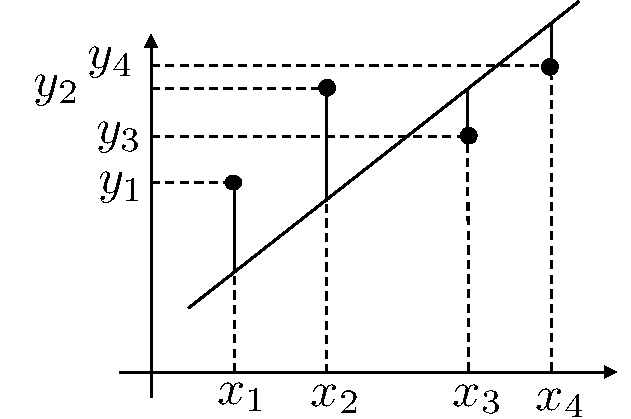
\includegraphics[width=0.5\textwidth]
			{figures/chap7_total_least_squares}
	\end{center}
	In other words: fix the $x_i$'s and play with $a$ to minimize the error.	
\end{frame}

%----------------------------------
\begin{frame}\frametitle{Application:  Total least squares}
	For the general problem $\min \norm{Ax - b}$ we assume $A$ is perfect and that the imperfection is completely in $b$
	\begin{center}
		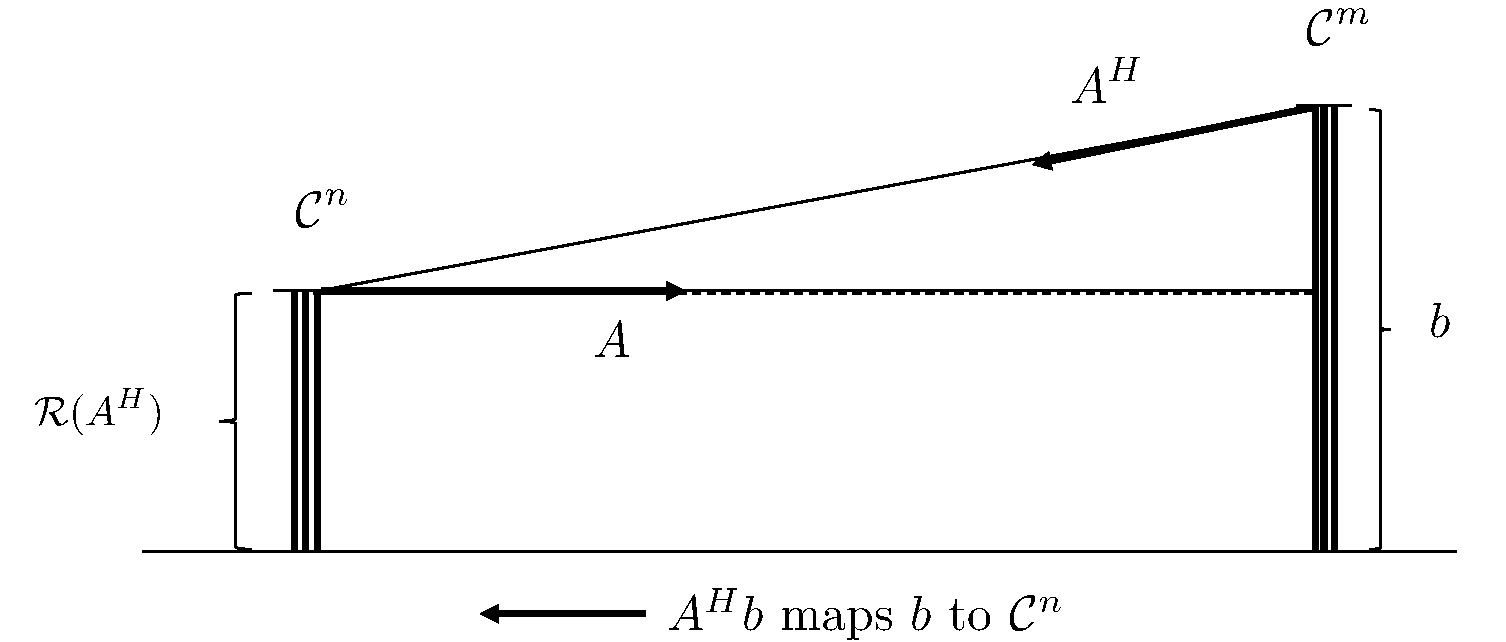
\includegraphics[width=0.5\textwidth]{figures/chap7_svd_2}
	\end{center}
	Recall $A^HAx = A^Hb$.  When we premultiply by $A^H$ we zero everything in $b$ that was in the null space of $A^H$ (i.e. we get rid of the bad parts of $b$).	
\end{frame}

%----------------------------------
\begin{frame}\frametitle{Application:  Total least squares}
	However $A$ often comes from noisy data as well (like when fitting a line to data) e.g. if $\ubf_i = ax_i+b$, then
	\[ 
		\begin{pmatrix}
	    	y_1\\
	    	\vdots\\
	    	\underbrace{y_n}_{\text{noisy}}
	  	\end{pmatrix} 
	  	= \begin{pmatrix}
	    	x_1 & 1\\
	    	\vdots & \vdots \\
	    	\underbrace{x_n}_{\text{noisy}} 
	    	& \underbrace{1}_{\text{perfect}}
	  	  \end{pmatrix}
	  	  \begin{pmatrix}
	    	a\\b
	  	  \end{pmatrix}
	\]	
\end{frame}

%----------------------------------
\begin{frame}\frametitle{Application:  Total least squares}
	Another interpretation of least squares is to find the \underline{smallest} perturbation of $b$, i.e., $\delta b$ such that
	\[ 
		Ax = b + \delta b 
	\] 
	where $b + \delta b \in \mathcal{R}(A)$.
	
	\vfill
	
	The total lest squares problem is to find the smallest perturbation of $b$ and $A$, denoted $\delta b$, $\delta A$ such that
	\[ 
		(A + \delta A)x = (b + \delta b) 
	\]
	supposing that $\begin{pmatrix} A & b \end{pmatrix}$ is full rank.
\end{frame}

%----------------------------------
\begin{frame}\frametitle{Application:  Total least squares}
	This can be written as
	\[ 
		\begin{pmatrix}
	    	A & b
	  	\end{pmatrix}
	  	\begin{pmatrix}
	    	x \\ -1
	  	\end{pmatrix}
	  + \begin{pmatrix}
	    	\delta A & \delta b
	  	\end{pmatrix}
	  	\begin{pmatrix}
	    	x \\-1
	  	\end{pmatrix} = 0
	\]
	or
	\[ 
		\begin{bmatrix}
			\begin{pmatrix}
	    		A & b
	  		\end{pmatrix} 
	  		+ 
	  		\begin{pmatrix}
	    		\delta A & \delta b
	  		\end{pmatrix}	
		\end{bmatrix}
		\begin{pmatrix}
	    	x\\-1
	  	\end{pmatrix} = 0.
	\] 	
	Define
	\[ 
		C \defeq \begin{pmatrix}
	    			A  & b
	  			 \end{pmatrix}
	  	\text{ and } 
	  	\Delta = \begin{pmatrix}
	    			\delta A & \delta b
	  			 \end{pmatrix}
	\]
	then 
	\[ 
		(C + \Delta)\begin{pmatrix}
	    				x \\ -1
	  				 \end{pmatrix} = 0.
	\]
\end{frame}

%----------------------------------
\begin{frame}\frametitle{Application:  Total least squares}
	So 
	\(
		\begin{pmatrix}
	    	x \\ -1
	  	\end{pmatrix} \in \mathcal{N}(C+\Delta) 
	\)
	which implies that $C + \Delta$ 
	is not full rank.	
	
	\vfill
	
	The problem is then to find the smallest perturbation $\Delta$ such that $C+\Delta$ looses rank.
	
	\vfill
	
	Note that since
	\(
		C = \begin{pmatrix}
	    		A & b
	  		\end{pmatrix}
	  	\in \mathbb{C}^{m\times (n+1)},
	\) 
	for $C$ to be full rank, we must have that $m>n$. 
	Therefore we can write
	\[
		C = \sum_{j=1}^{n+1}\sigma_j\ubf_j\vbf_j^H.
	\]
\end{frame}

%----------------------------------
\begin{frame}\frametitle{Application:  Total least squares}
	Hence, the smallest $\Delta$ that reduces the rank of $C$ is 
	\[
		\Delta = -\sigma_{n+1}\ubf_{n+1}\vbf_{n+1}^H.
	\]
	
	\vfill
	
	Note that $\vbf_{n+1} \in \mathcal{N}(C+\Delta)$ 
	since
	\[ 
		(C+\Delta)\vbf_{n+1} 
			= \sum_{j=1}^r\sigma_j\ubf_j\vbf_j^H\vbf_{n+1} 
			= 0
	\]
	since $\vbf_i\vbf_j = \delta_{ij}$. 
\end{frame}

%----------------------------------
\begin{frame}\frametitle{Application:  Total least squares}
	Therefore
	\begin{align*}
		\begin{pmatrix}
	    	x\\ -1
	  	\end{pmatrix} 
	  		= \alpha \vbf_{n+1} 
	  		= \alpha \begin{pmatrix}
	    				\vbf_{n+1}(n:1)\\
	    				\vbf_{n+1}(n+1)
	  			 	  \end{pmatrix}
	\end{align*}
	Letting $\alpha = -\frac{1}{\vbf_{n+1}(n+1)}$ gives
	\[
	x = \alpha \vbf_{n+1}(n:1)
	\]
	
	\vfill
	
	This is valid if $\vbf_{n+1}(n+1) \neq 0$.  Note that if $\sigma_{n+1}$ is not a unique minimum singular value, i.e. $\sigma_{n+1} = \sigma_n = \cdots = \sigma_{k+1}$ then we want to find the smallest norm $x$ such that
	\[ 
	\begin{pmatrix}
	    x\\ -1
	  \end{pmatrix} \in span\{ \vbf_{k+1},\ldots,\vbf_{n+1} \} 
	 \]	
\end{frame}

%----------------------------------
\begin{frame}\frametitle{Application:  Homography Matrix}
	
\end{frame}


%%----------------------------------
%\begin{frame}\frametitle{Application:  MIMO Feedback Control}
%	Consider the MIMO feedback system shown below:
%	\begin{center}
%		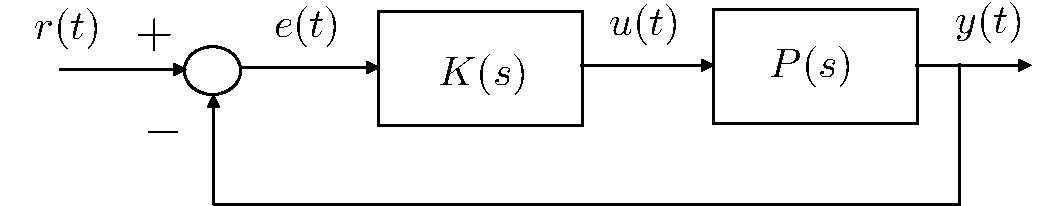
\includegraphics[width=0.9\textwidth]{figures/chap7_svd_feedback}
%	\end{center}	
%	The transfer matrix is derived by noting that
%	\begin{align*}
%		& E = R-Y = R-PU = R-PKE \\
%		\implies & E + PKE = R \\
%		\implies & (I + PK) E = R \\
%		\implies & 	E(s) = (I-PK)^{-1}R(s) \\
%	\end{align*}
%\end{frame}
%
%%----------------------------------
%\begin{frame}\frametitle{Application:  MIMO Feedback Control}
%	Taking the norm of $E(s)$ gives
%	\begin{align*}
%		\norm{E(s)} 
%			&= \norm{(I-PK)^{-1}R(s)} \\
%			&\leq \norm{(I-PK)^{-1}}\norm{R(s)} \\
%			&= \frac{1}{\underline{\sigma}(I-PK)}\norm{R(j\omega)},
%	\end{align*}
%	where $\underline{\sigma}(I-PK)(s)$ is the smallest singular value of $I-P(s)K(s)$.
%
%
%
%
%
%	\[ \norm{(I - PK)^{-1} } \]
%	\[ \norm{A^{-1} } = \frac{1}{\sigma(I-PK)} \]
%	\newpage
%	want
%	
%	\begin{align*}
%	\vec{\sigma}((I+PK)^{-1}) &\leq \gamma(j\omega)\\
%	= \frac{1}{\sigma(I+PK)} &\leq \gamma(j\omega)\\
%	\frac{1}{\gamma(j\omega)} &\leq \sigma(I+PK) \leq \sigma(I) + \vec{sigma}(PK)\\
%	&= 1 + \vec{\sigma}(PK)\\
%	\therefore \vec{\sigma}(PK) \leq \frac{1}{\gamma(j\omega)} - 1
%	\end{align*}
%	
%	
%	use the fact that
%	\[ \sigma(Q+R) \leq \sigma(Q) + \vec{\sigma}(R) \]
%	
%\end{frame}

%----------------------------------
\begin{frame}\frametitle{Application:  MIMO Communication}
	Consider the MIMO communication system modeled by
	\[ 
		\underbrace{
			Y(j\omega)
		}_{p\times 1} 
		= \underbrace{
			H(j\omega)
		  }_{1\times m}
		  \underbrace{
		  	X(j\omega)
		  }_{m\times 1} 
	\]
	
	\vfill
	
	What is the maximum gain of the system?
	\begin{align*}
		\norm{Y(j\omega)} 
			= \norm{H(j\omega)X(j\omega)} 
			\leq \norm{H(j\omega)}\norm{X(j\omega)} 
	\end{align*}
	Therefore, the maximum gain is given by
	\begin{align*}
		\gamma_{\max}(j\omega) 
			&=  \max_{X(j\omega) \neq 0}
					\frac{\norm{H(j\omega)X(j\omega)}}{\norm{X(j\omega)}} \\
		&= \norm{H(j\omega)}\\
		&= \bar{\sigma}(H(j\omega)),
	\end{align*}
	where $\bar{\sigma}(H(j\omega))$ is the maximum singular value of $H(j\omega)$.
\end{frame}

%----------------------------------
\begin{frame}\frametitle{Application:  MIMO Communication}
	How do you achieve this gain?
	Since 
	\[
		H(j\omega) 
			= \Sigma \sigma_k(j\omega)\ubf_k(j\omega)\vbf_k^H(j\omega),
	\]
	letting
	\[ 
		X(j\omega) = \vbf_1(j\omega) 
	\]
	maximizes the gain in the system over the set 
	$\norm{X(j\omega) } = 1$	.
\end{frame}

\end{document}
